\problem{Problem 3}
\emph{The Fourier solution of the initial value problem}
\begin{align*}
    &\begin{array}{lll}
        u_{tt} = u_{xx}, &0 < x < 1, & t > 0, \\
        u(0, t) = 0, & u(1, t) = 0, & t > 0
    \end{array} \\
    &u(x,0) = \begin{cases}
        2x & \text{ if } 0 \leq x \leq \frac{1}{2} \\
        2(1-x) & \text{ if } \frac{1}{2} < x < 1
    \end{cases}, \\
    &= u_t(x,0) = 0, \qquad 0 \leq x \leq 1
\end{align*}
\emph{is given by $$u(x,t) = \frac{8}{\pi^2}\sum_{n=1}^\infty \frac{(-1)^{n+1}}{(2n-1)^2}\sin\qty[(2n-1)\pi x]\cos\qty[(2n-1)\pi t]$$}
\begin{enumerate}[\bf (a)]
    \item
        \emph{Show that the Fourier seires converges to a continuous function.  How many spacial (weak) $L^2$-derivatives does $u(x,t)$ have?} \\

        For a fixed $t$, it suffices to show the partial sums $u_N$ converge to a function in $H^k$ for $k < \frac{3}{2}$ (and $u \not\in H^k$ for $k \geq \frac{3}{2}$) where $H^k$ is the Sobolev space of order $k$.  Then by the Sobolev Embedding Theorem, $u$ converges to a continuous function.  Thus, that continuous function has a weak spacial $L^2$ derivative $u' \not\in H^{\frac{1}{2}}$, and so $u$ does not have two weak spacial derivatives.

        To show this is true, fix $t$ and denote $c_t = \cos\qty[\qty(2n-1)\pi t] \in \Rl$.  Then the Fourier coefficients $\hat{u}_n$ are proportional to the following (we do not say equal since we want to consider the standard Fourier basis $\left\{e^{inx}\right\}_{n\in\mathbb{Z}}$ as opposed to the basis $\big\{1, \sin nx, \cos nx\big\}_{n=1}^\infty$).
        \begin{align*}
            \left|\hat{u}_n\right| \propto \frac{1}{(2n-1)^2} \qquad \text{and} \qquad \sum_{n=1}^\infty \hat{u}_n^2 \propto \sum_{n=1}^\infty \frac{1}{n^4}
        \end{align*}
        which converges.  Then the Fourier coefficients of the weak derivative are proportional to the following:
        \begin{align*}
            \left|\hat{u'}_n\right| = \left|n\hat{u}_n\right| \propto \frac{n}{(2n-1)^2} \qquad \text{and} \qquad \sum_{n=1}^\infty \hat{u'}_n^2 \propto \sum_{n=1}^\infty \frac{1}{n^2}
        \end{align*}
        which also conveges.  However,
        \begin{align*}
            \left|\hat{u''}_n\right| = \left|n^2\hat{u}_n\right| \propto \frac{n^2}{(2n-1)^2} \qquad \text{and} \qquad \sum_{n=1}^\infty \hat{u''}_n^2 \propto \sum_{n=1}^\infty 1
        \end{align*}
        which diverges.
    \item
        \emph{Verify from the Fourier solution that $$\int_0^1\qty[u_t^2(x,t) + u_x^2(x,t)]\dd x = \text{constant} \qquad \text{ for } -\infty < t < \infty.$$}

        First note
        \begin{align*}
            u_x(x,t) = \frac{8}{\pi^2}\sum_{n=1}^\infty \frac{(-1)^{n+1}}{(2n-1)^2}(2n-1)\pi\cos\qty((2n-1)\pi x)\cos\qty((2n-1)\pi t), \qquad \text{and} \\
            u_t(x,t) = \frac{8}{\pi^2}\sum_{n=1}^\infty \frac{(-1)^n}{(2n-1)^2}(2n-1)\pi\sin\qty((2n-1)\pi x)\sin\qty((2n-1)\pi t)
        \end{align*}
        and since
        \begin{align*}
            \int_0^1 \cos((2n-1)\pi x)\cos((2m-1)\pi x)\dd x = \int_0^1 \sin((2n-1)\pi x)\sin((2m-1)\pi x)\dd x = \frac{1}{2}\delta_{n,m} = \begin{cases}
                \frac{1}{2} & \text{ if } n = m\\
                0 & \text{ if } n \neq m
            \end{cases}
        \end{align*}
        then
        \begin{align*}
            \int_0^1 u_t^2 \dd x &= \frac{64}{\pi^2}\sum_{n=1}^\infty \frac{1}{(2n-1)^2}\sin^2((2n-1)\pi t)\int_0^1\sin^2((2n-1)\pi x)\dd x, \qquad \text{and} \\
            \int_0^1 u_x^2 \dd x &= \frac{64}{\pi^2}\sum_{n=1}^\infty \frac{1}{(2n-1)^2}\cos^2((2n-1)\pi t)\int_0^1\cos^2((2n-1)\pi x)\dd x \\
            \implies \int_0^1 \qty[u_t^2 + u_x^2]\dd x & \\
            = \frac{64}{\pi^2}\sum_{n=1}^\infty \frac{1}{(2n-1)^2}&\qty[\sin^2((2n-1)\pi t)\int_0^1 \sin^2((2n-1)\pi x)\dd x + \cos^2((2n-1)\pi t)\int_0^1 \cos^2((2n-1) \pi x)\dd x] \\
            &= \frac{32}{\pi^2}\sum_{n=1}^\infty \frac{1}{(2n-1)^2}\qty[\sin^2((2n-1)\pi t) + \cos^2((2n-1)\pi t)] \\
            &= \frac{32}{\pi^2}\sum_{n=1}^\infty \frac{1}{(2n-1)^2} \\
            &= \frac{32}{\pi^2}\cdot\frac{\pi^2}{8} \\
            &= 4
        \end{align*}
    \item
        \emph{Use \texttt{MATLAB} (or another program) to compute the partial sum $$u_N(x,t) = \frac{8}{\pi^2}\sum_{n=1}^N\frac{(-1)^{n+1}}{(2n-1)^2}\sin\qty[(2n-1)\pi x]\cos\qty[(2n-1)\pi t]$$ at $t = 0.25$ for $N = 5$ and $N = 50$.}
        \begin{center}
            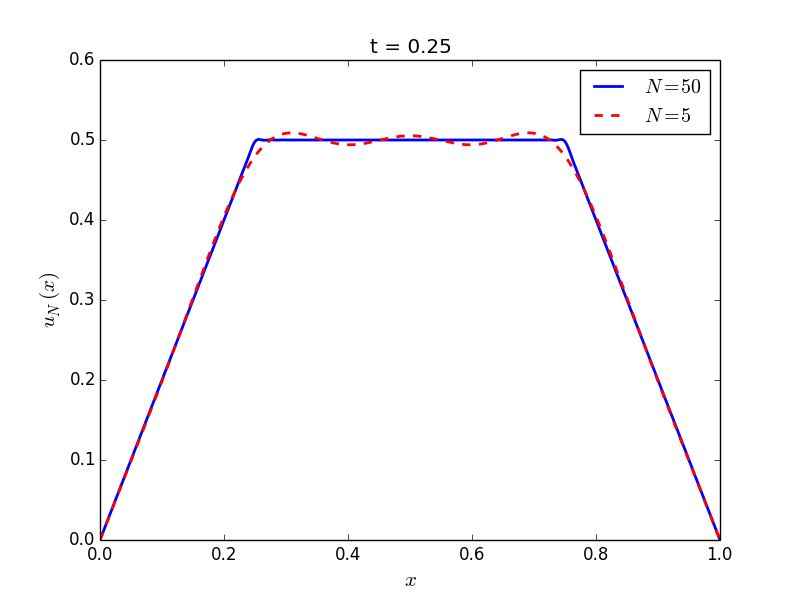
\includegraphics[scale=0.75]{problem_3c.png}
        \end{center}
    \item
        \emph{Use the addition formula for sines to show that the Fourier solution can be written in the form of the d'Alembert solution as $$u(x,t) = F(x - t) + F(x + t)$$ for a suitable function $F\ :\ \Rl \rightarrow \Rl$.  What is $F$?} \\

        Define $\tilde{F}$ as half the initial data, i.e.
        \begin{align*}
            \tilde{F}(x) = \begin{cases}
                x & \text{ if } 0 \leq x \leq n + \frac{1}{2} \\
                1 - x & \text{ if } \frac{1}{2} < x < 1
            \end{cases}
        \end{align*}
        Let $F$ be it's odd $2$-periodic expansion,
        \begin{align*}
            F(x) = \begin{cases}
                x & \text{ if } n - \frac{1}{2} \leq x \leq n + \frac{1}{2} \\
                1 - x & \text{ if } n + \frac{1}{2} < x < n + \frac{3}{2}
            \end{cases} \qquad \frac{n}{2} \in \mathbb{Z}
        \end{align*}
        and note its Fourier series representation:
        \begin{align*}
            F(x) = \frac{4}{\pi^2}\sum_{n=1}^\infty \frac{(-1)^{n+1}}{(2n-1)^2}\sin((2n-1)\pi x)
        \end{align*}
        Then note $F(x - t) + F(x + t) = u(x,t)$ because
        \begin{align*}
            F(x - t) + F(x + t) &= \frac{4}{\pi^2}\sum_{n=1}^\infty \frac{(-1)^{n+1}}{(2n-1)^2}\sin((2n-1)\pi (x - t)) + \frac{4}{\pi^2}\sum_{n=1}^\infty \frac{(-1)^{n+1}}{(2n-1)^2}\sin((2n-1)\pi (x + t)) \\
            &= \frac{8}{\pi^2}\sum_{n=1}^\infty \frac{(-1)^{n+1}}{(2n-1)^2}\frac{1}{2}\qty[\sin((2n-1)\pi(x-t)) + \sin((2n-1)\pi(x+t))] \\
            &= \frac{8}{\pi^2}\sum_{n=1}^\infty \frac{(-1)^{n+1}}{(2n-1)^2}\sin((2n-1)\pi x)\cos((2n-1)\pi t) \\
            &= u(x,t)
        \end{align*}
\end{enumerate}